\documentclass[12pt, titlepage]{article}

\usepackage{fullpage}
\usepackage[round]{natbib}
\usepackage{multirow}
\usepackage{booktabs}
\usepackage{tabularx}
\usepackage{graphicx}
\usepackage{float}
\usepackage{hyperref}
\hypersetup{
    colorlinks,
    citecolor=black,
    filecolor=black,
    linkcolor=red,
    urlcolor=blue
}
\usepackage[round]{natbib}

\newcounter{acnum}
\newcommand{\actheacnum}{AC\theacnum}
\newcommand{\acref}[1]{AC\ref{#1}}

\newcounter{ucnum}
\newcommand{\uctheucnum}{UC\theucnum}
\newcommand{\uref}[1]{UC\ref{#1}}

\newcounter{mnum}
\newcommand{\mthemnum}{M\themnum}
\newcommand{\mref}[1]{M\ref{#1}}

\title{SE 3XA3: Module Guide\\PasswordProtectionProgram}

\author{Team 28, Tuples1
		\\ Suhavi Sandhu (sandhs11)
		\\ Shabana Dhayananth (dhayanas)
		\\ Joseph Lu (luy89)
}

\date{\today}

\begin{document}

\maketitle

\pagenumbering{roman}
\tableofcontents
\listoftables
\listoffigures

\begin{table}[bp]
\caption{\bf Revision History}
\begin{tabularx}{\textwidth}{p{3cm}p{2cm}X}
\toprule {\bf Date} & {\bf Version} & {\bf Notes}\\
\midrule
2017-11-10 & 0.0 & Creation\\
\bottomrule
\end{tabularx}
\end{table}

\newpage

\pagenumbering{arabic}

\section{Introduction}\label{Intro}

\subsection{Brief Project Overview} \label{ProjOver}
The purpose of this project is to implement an encrypted password manager, PasswordProtectionProgram (PPP) wherein a person can 
safely store and access all of the passwords they use with a single master password. Through working on this project the software 
team also hopes to learn about encryption methods and the development process.

\subsection{Document Overview} \label{DocOver}
This document specifies the modular structure of the system, the 
PasswordProtectionProgram, and is intended to allow both designers and 
maintainers to easily identify the parts of the software. The document 
shall act as a guide for new project members that want to understand 
the system, a hierarchical structure for maintainers that want to 
improve the system, and a source for designers to verify the system’s 
consistency, feasibility and flexibility.

The document is organized such that the anticipated and unlikely 
changes of the software requirements are listed, following a 
summarization of the module decomposition that has been constructed 
keeping the likely changes in mind. Next, the connections between 
software requirements and modules are given along with a detailed 
description of the modules. The document also includes 2 traceability 
matrices, one that checks for completeness of the design against the 
requirements from the SRS and another that shows the relation between 
anticipated changes and the modules. Lastly there is the use relation 
between modules.


\section{Anticipated and Unlikely Changes} \label{SecChange}

This section lists possible changes to the system. According to the likeliness
of the change, the possible changes are classified into two
categories. Anticipated changes are listed in Section \ref{SecAchange}, and
unlikely changes are listed in Section \ref{SecUchange}.

\subsection{Anticipated Changes} \label{SecAchange}

Anticipated changes are the source of the information that is to be hidden
inside the modules. Ideally, changing one of the anticipated changes will only
require changing the one module that hides the associated decision. The approach
adapted here is called design for change.

\begin{description}
  \item[\refstepcounter{acnum} \actheacnum \label{acInput}:] The operating system
  that the application is being run on.
  \item[\refstepcounter{acnum} \actheacnum \label{acFramework}:] The framework for
  the graphical user interface.
  \item[\refstepcounter{acnum} \actheacnum \label{acDatabase}:] The database management system that is ued to store sensitive information.
  \item[\refstepcounter{acnum} \actheacnum \label{acEncryption}:] The encryption library that secures user information.
  \item[\refstepcounter{acnum} \actheacnum \label{acUserCustom}:] Customization functionality for the user (ex. change the inactivity time before the application logs out).
  \item[\refstepcounter{acnum} \actheacnum \label{acDBAttributes}:] The attributes of the database.
  \item[\refstepcounter{acnum} \actheacnum \label{acPassGenFunc}:] Additional functionality from password generator (ex. constraining the random password to have only numbers, special characters).
  \item[\refstepcounter{acnum} \actheacnum \label{acPortability}:] The portability of the application (ex. allow the application to be used online).
\end{description}

\subsection{Unlikely Changes} \label{SecUchange}

The module design should be as general as possible. However, a general system is
more complex. Sometimes this complexity is not necessary. Fixing some design
decisions at the system architecture stage can simplify the software design. If
these decision should later need to be changed, then many parts of the design
will potentially need to be modified. Hence, it is not intended that these
decisions will be changed.

\begin{description}
  \item[\refstepcounter{ucnum} \uctheucnum \label{ucIO}:] Input/Output devices
  used by the system.
  \item[\refstepcounter{ucnum} \uctheucnum \label{ucInput}:] The input to the 
  system will always be external.
  \item[\refstepcounter{ucnum} \uctheucnum \label{ucDBase}:] The use of a database to store the user data.
  \item[\refstepcounter{ucnum} \uctheucnum \label{ucPassEncrypt}:] Individual encryption of each password input to the system.
  \item[\refstepcounter{ucnum} \uctheucnum \label{ucPurpose}:] The goal of the system is provide a secure storage of the user's passwords.
  \item[\refstepcounter{ucnum} \uctheucnum \label{ucLanguage}:] The development language that is used.

\end{description}

\section{Module Hierarchy} \label{SecMH}

This section provides an overview of the module design. Modules are summarized
in a hierarchy decomposed by secrets in Table \ref{TblMH}. The modules listed
below, which are leaves in the hierarchy tree, are the modules that will
actually be implemented.

\begin{description}
  \item [\refstepcounter{mnum} \mthemnum \label{mIn}:] Input Module
  \item [\refstepcounter{mnum} \mthemnum \label{mPG}:] Password Generator Module
  \item [\refstepcounter{mnum} \mthemnum \label{mEH}:] Encryption Handling Module
  \item [\refstepcounter{mnum} \mthemnum \label{mPCUC}:] Password Checking Upon Creation Module
  \item [\refstepcounter{mnum} \mthemnum \label{mPCUL}:] Password Checking Upon Login Module
  \item [\refstepcounter{mnum} \mthemnum \label{mGUI}:] GUI Module
  \item [\refstepcounter{mnum} \mthemnum \label{mCop}:] Copy Module
  \item [\refstepcounter{mnum} \mthemnum \label{mInac}:] Inactivity Module
  \item [\refstepcounter{mnum} \mthemnum \label{mDB}:] Database Module
  \item [\refstepcounter{mnum} \mthemnum \label{mCons}:] Constants Module

\end{description}

\textbf{Note:} The implentation of PasswordProtectionProgram is completely software based, therefore there are no relevant hardware hiding modules.

\begin{table}[h!]
\centering
\begin{tabular}{p{0.3\textwidth} p{0.6\textwidth}}
\toprule
\textbf{Level 1} & \textbf{Level 2}\\
\midrule

{Hardware-Hiding Module} & ~ \\
\midrule

\multirow{7}{0.3\textwidth}{Behaviour-Hiding Module} 
& Input Module\\
& Password Generator Module\\
& Encryption Handling Module\\
& GUI Module\\
& Copy Module\\
& Database Module\\ 
\midrule

\multirow{3}{0.3\textwidth}{Software Decision Module} 
& Password Checking Upon Creation\\
& Password Checking Upon Login Module\\
& Inactivity Module\\
& Constants Module\\
\bottomrule

\end{tabular}
\caption{Module Hierarchy}
\label{TblMH}
\end{table}

\section{Connection Between Requirements and Design} \label{SecConnection}

The system was designed to satisfy the requirements that were developed in the Software Requirement Specification. The GUI module will satisfy all the visibility and usability requirements as it is the module to deal with the user’s ability to see and use the application. This module also satisfies many functional requirements of the SRS. The Encryption module satisfies security requirements. The database module satisfies many functional as well as security requirements. The connection between requirements and modules is listed in Table \ref{TblRT}.

\section{Module Decomposition} \label{SecMD}

Modules are decomposed according to the principle of ``information hiding''
proposed by \citet{ParnasEtAl1984}. The \emph{Secrets} field in a module
decomposition is a brief statement of the design decision hidden by the
module. The \emph{Services} field specifies \emph{what} the module will do
without documenting \emph{how} to do it. For each module, a suggestion for the
implementing software is given under the \emph{Implemented By} title. If the
entry is \emph{OS}, this means that the module is provided by the operating
system or by standard programming language libraries.  Also indicate if the
module will be implemented specifically for the software.

Only the leaf modules in the
hierarchy have to be implemented. If a dash (\emph{--}) is shown, this means
that the module is not a leaf and will not have to be implemented. Whether or
not this module is implemented depends on the programming language
selected.

\subsection{Hardware Hiding Modules}

Not applicable as the system is software-based and the lowest level that the software interfaces with is the Operating System..

\subsection{Behaviour-Hiding Module}

\subsubsection{Input Module (\mref{mIn})}

\begin{description}
\item[Secrets:] The format and structure of the input data.
\item[Services:] Converts the input data into the data structure used by the
  input parameters module.
\item[Implemented By:] PasswordProtectionProgram
\end{description}

\subsubsection{Password Generator Module (\mref{mPG})}

\begin{description}
\item[Secrets:] The algorithm used to generate random password.
\item[Services:] Creates a random 8 character password consisting of uppercase letters, lowercase letters and numerical values.
\item[Implemented By:] PasswordProtectionProgram and Python Libraries
\end{description}

\subsubsection{Encrytion Handling Module (\mref{mEH})}

\begin{description}
\item[Secrets:] The algorithm used to generate the key to encrypt the password.
\item[Services:] Creates a key using PBKDF2HMAC and Python's cryptography library, Fernet. That key is then used to encrypt and decrypt inputs.
\item[Implemented By:] PasswordProtectionProgram and Python Libraries (Fernet)
\end{description}

\subsubsection{GUI Module (\mref{mGUI})}

\begin{description}
\item[Secrets:] The structure and processing of user input.
\item[Services:] Takes in user input data and verifies it if necessary. Stores data into and retrieves data from the database to display.
\item[Implemented By:] PasswordProtectionProgram and Python Libraries (tkinter)
\end{description}

\subsubsection{Copy Module (\mref{mCop})}

\begin{description}
\item[Secrets:] The cross platform to copy text to clipboard.
\item[Services:] Copies user's selected username and password as text to clipboard.
\item[Implemented By:] PasswordProtectionProgram and Python Libraries (pyperclip)
\end{description}

\subsubsection{Database Module (\mref{mDB})}

\begin{description}
\item[Secrets:] Database Management System structure used to store and retrieve data.
\item[Services:] Stores and retrieves entry information such as account name, account type, username, hash value, hash key.
\item[Implemented By:] PasswordProtectionProgram and Python Libraries (peewee)
\end{description}


\subsection{Software Decision Module}

\subsubsection{Password Check Upon Creation (\mref{mPCUC})}

\begin{description}
\item[Secrets:] The algorithm used to check the created master password.
\item[Services:] Informs user if the password is missing key elements, such as upper and lower case letters, a number, a special character, and a minimum length of 8.
\item[Implemented By:] PasswordProtectionProgram and Python Libraries (re)
\end{description}

\subsubsection{Password Check Upon Login (\mref{mPCUL})}

\begin{description}
\item[Secrets:] The algorithm used to verify that the user entered the correct master password.
\item[Services:] Verifies input password against one stored in database.
\item[Implemented By:] PasswordProtectionProgram and Python Libraries (re)
\end{description}

\subsubsection{Inactivity Module (\mref{mInac})}

\begin{description}
\item[Secrets:] The algorithm used to detect user inactivity.
\item[Services:] Logs user out of account after a certain period of inactivity.
\item[Implemented By:] PasswordProtectionProgram
\end{description}

\subsubsection{Constants Module (\mref{mCons})}

\begin{description}
\item[Secrets:] The style parameters used to characterize the physical display of the application.
\item[Services:] Constants defining the window size, colour scheme, and fonts.
\item[Implemented By:] PasswordProtectionProgram
\end{description}

\section{Traceability Matrix} \label{SecTM}

This section shows two traceability matrices: between the modules and the
requirements and between the modules and the anticipated changes.

% the table should use mref, the requirements should be named, use something
% like fref
\begin{table}[H]
\centering
\begin{tabular}{p{0.2\textwidth} p{0.6\textwidth}}
\toprule
\textbf{Req.} & \textbf{Modules}\\
\midrule
FR1 & \mref{mCons}\\
FR2 & \mref{mDB}\\
FR3 & \mref{mPCUC}\\
FR4 & \mref{mPCUL}\\
FR5 & \mref{mIn}, \mref{mGUI}\\
FR6 & \mref{mPG}\\
FR7 & \mref{mGUI}\\
FR8 & \mref{mEH}, \mref{mDB}\\
FR9 & \mref{mCop}\\
FR10 & \mref{mPCUC}\\
FR11 & \mref{mEH}\\
\bottomrule
\end{tabular}
\caption{Trace Between Functional Requirements and Modules}
\label{TblRT}
\end{table}

\begin{table}[H]
\centering
\begin{tabular}{p{0.2\textwidth} p{0.6\textwidth}}
\toprule
\textbf{Req.} & \textbf{Modules}\\
\midrule
NFR1 & \mref{mGUI}\\
NFR2 & \mref{mIn}, \mref{mGUI}\\
NFR3 & \mref{mIn}, \mref{mGUI}\\
NFR7 & \mref{m}\\
NFR9 & \mref{mIn}, \mref{mGUI}\\
NFR11 & \mref{mCons}, \mref{mGUI}\\
NFR12 & \mref{mCons}, \mref{mGUI}\\
NFR13 & \mref{mIn}\\
NFR15 & \mref{mEH}, \mref{mDB}\\
NFR16 & \mref{mEH}, \mref{mPCUL}\\
NFR17 & \mref{mInac}\\
\bottomrule
\end{tabular}
\caption{Trace Between Non-Functional Requirements and Modules}
\label{TblRT}
\end{table}

\begin{table}[H]
\centering
\begin{tabular}{p{0.2\textwidth} p{0.6\textwidth}}
\toprule
\textbf{AC} & \textbf{Modules}\\
\midrule
\acref{acInput} & \mref{mIn}\\
\acref{acFramework} & \mref{mGUI}\\
\acref{acDatabase} & \mref{mDB}\\
\acref{acEncryption} & \mref{mEH}\\
\acref{acUserCustom} & \mref{mCons}\\
\acref{acDBAttributes} & \mref{mDB}\\
\acref{acPassGenFunc} & \mref{mPG}\\
\acref{acPortability} & \mref{mGUI}\\
\bottomrule
\end{tabular}
\caption{Trace Between Anticipated Changes and Modules}
\label{TblACT}
\end{table}

\section{Use Hierarchy Between Modules} \label{SecUse}

In this section, the uses hierarchy between modules is
provided. \citet{Parnas1978} said of two programs A and B that A {\em uses} B if
correct execution of B may be necessary for A to complete the task described in
its specification. That is, A {\em uses} B if there exist situations in which
the correct functioning of A depends upon the availability of a correct
implementation of B.  Figure \ref{FigUH} illustrates the use relation between
the modules. It can be seen that the graph is a directed acyclic graph
(DAG). Each level of the hierarchy offers a testable and usable subset of the
system, and modules in the higher level of the hierarchy are essentially simpler
because they use modules from the lower levels.

\begin{figure}[H]
\centering
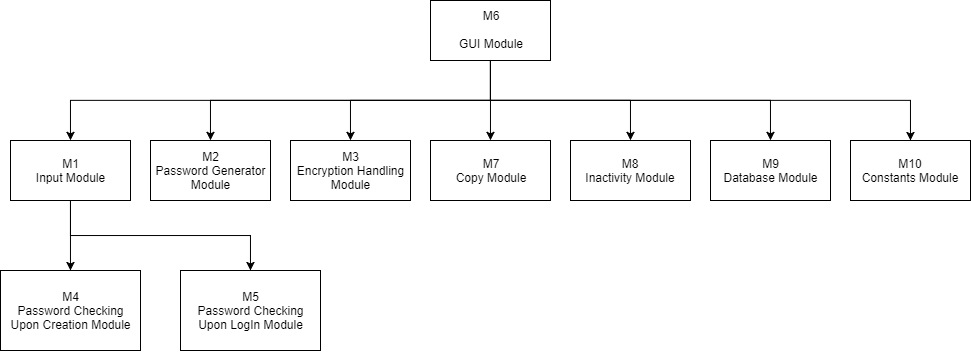
\includegraphics[scale=0.5]{Images/DAG.png}
\caption{Use hierarchy among modules}
\label{FigUH}
\end{figure}

%\section*{References}

\bibliographystyle {plainnat}
\bibliography {MG}

\end{document}